\section{楕円解析幾何学}

楕円解析幾何学は、双曲解析幾何学を展開したのとまったく同じように展開でき、公式は因子 $i$ を除いたものと同じになる。しかしこれらの公式は、直線と極の関係からも非常に容易に得られるから、そのようにして導く。

楕円平面解析幾何学の公式は、三つの幾何学のどれにおいても、球面に適用できる。

\begin{figure}[h]
\centering
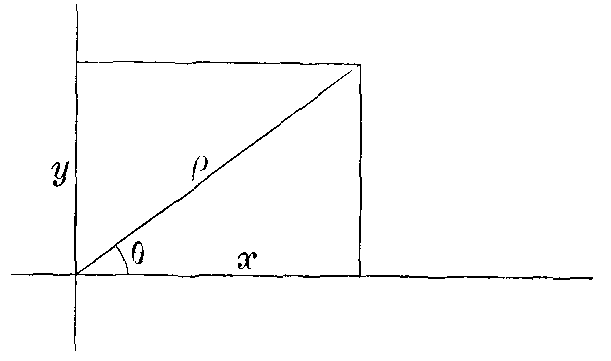
\includegraphics[width=60mm]{fig72.png}
\end{figure}

\begin{description}
\item[1.~極座標と直交座標の関係:]

\begin{gather*}
\tan x = \cos\theta\, \tan\rho, \quad \tan y = \sin\theta\, \tan\rho; \\
\intertext{したがって、}
\begin{aligned}
  \tan^2\rho &= \tan^2x + \tan^2y,\\
  \tan\theta &= \frac{\tan y}{\tan x}.\footnotemark
\end{aligned}
\end{gather*}
\footnotetext{原点を極とする直線は、座標軸とともに三直角三角形をつくり、$x$、$y$、$\theta$ は、与えられた点のそれらの三つの頂点からの方向を表すとみなしてよい。
\par 球面上で、赤道の極を原点にとれば、$\rho$ と $\theta$ は余緯度と経度である。$x$ と $y$ は、一方は符号を変えて、赤道上の $90^\circ$ 離れた二点からのその点の「方位」である。}

\begin{figure}[h]
\centering
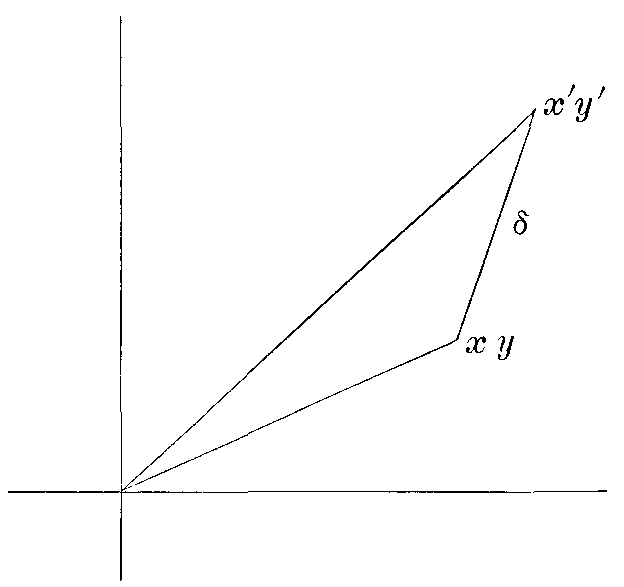
\includegraphics[width=60mm]{fig74.png}
\end{figure}

\item[2.~二点間の距離 \boldmath$\delta$:]

\begin{equation*}
\cos\delta = \cos\rho\,\cos\rho' +
                             \sin\rho\,\sin\rho'\cos(\theta'-\theta).
\end{equation*}

これは、$\rho'$ と $\theta'$ を中心の極座標とする、半径 $\delta$ の円の極方程式とみなせる。

さて、
\begin{align*}
  \sin\rho\,\cos\theta &= \cos\rho\,\tan x,\\
  \sin\rho\,\sin\theta &= \cos\rho\,\tan y;
\intertext{また、}
  \cos\rho = \frac{1}{\sqrt{1+\tan^2\rho}}
  &= \frac{1}{\sqrt{1+\tan^2x+\tan^2y}}
\end{align*}
したがって、円の直交座標による方程式は次のように書ける。
\begin{multline*}
  (1 + \tan^2x + \tan^2y) (1 + \tan^2x' + \tan^2y') \cos^2\delta\\
  = (1 + \tan x\tan x' + \tan y\tan y')^2.
\end{multline*}

\begin{figure}[h]
\centering
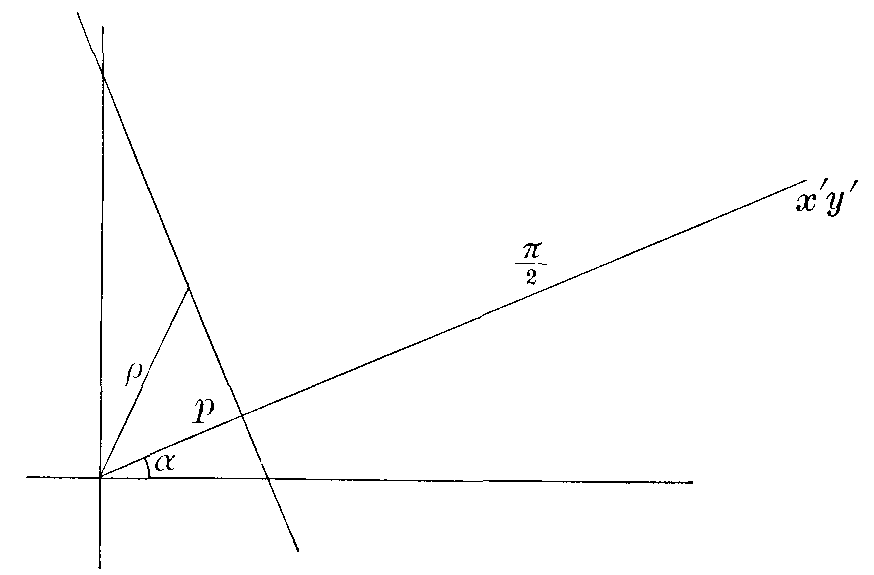
\includegraphics[width=60mm]{fig75.png}
\end{figure}

\item[3.~直線の方程式:]\hfill\break

$\delta = \frac{\pi}{2}$ のとき、円は直線になる。したがってこの場合は、方程式
\begin{equation*}
  \tan x \tan x' + \tan y \tan y' + 1 = 0
\end{equation*}
を得る。$x'y'$ は直線の極である。

方程式
\begin{align*}
\tan\rho\, \cos(\theta-\alpha) &= \tan p, \\
\intertext{すなわち}
\cos\alpha\, \tan x + \sin\alpha\,\tan y &= \tan p, \\
\intertext{から}
\tan x' &= -\frac{\cos\alpha}{\tan p},\\
\tan y' &= -\frac{\sin\alpha}{\tan p}
\end{align*}
を得る。これは幾何学的に示すこともでき、この点の極座標は
\begin{equation*}
p+\frac{\pi}{2},\ \alpha
\end{equation*}
である。

方程式
\begin{equation*}
  a\tan x + b\tan y + 1 = 0
\end{equation*}
は、$a$ と $b$ の任意の実数値に対して、実の直線を表す。

\item[4.~点から直線までの距離 \boldmath$\delta$:]\hfill\break

これは、その点と直線の極との間の距離の余角である。次の方程式で表される。
\begin{align*}
  \sin\delta &= -\cos\rho\,\sin p
                            + \sin\rho\,\cos p\,\cos(\theta-\alpha)\\
  &= \cos\rho\,\cos p
                 \left[\tan\rho\,\cos(\theta-\alpha) - \tan p\right].
\end{align*}

\item[5.~二直線のなす角 \boldmath$\phi$:]\hfill\break

これはそれらの極の間の距離に等しい。したがって、
\begin{equation*}
  \cos\phi = \sin p\,\sin p' + \cos p\,\cos p'\,\cos(\alpha'-\alpha).
\end{equation*}

二直線
\begin{align*}
  a\phantom{'}\tan x + b\phantom{'}\tan y + 1 &= 0,\\
  a'\tan x + b'\tan y + 1 &= 0\\
  \intertext{が垂直であるのは、}
  aa' + bb' + 1 &= 0
\end{align*}
のときである。

\begin{figure}[h]
\centering
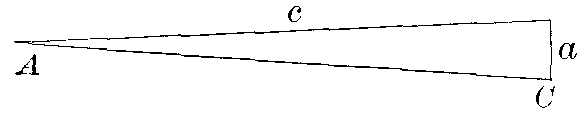
\includegraphics[width=60mm]{fig76.png}
\end{figure}

\item[6.~微分公式:]\hfill\break

公式
\begin{equation*}
  \frac{\sin A}{\sin a} = \frac{\sin C}{\sin c}
\end{equation*}
は、$A$ が限りなく小さくなるとき、
\begin{equation*}
  a = \sin c \cdot A\tag{I.}
\end{equation*}
となる。

\textbf{系.} \emph{半径 $\mathbf{r}$ の円において、任意の弧と、中心で張る角との比は $\sin \mathbf{r}$ である。}

\begin{figure}[h]
\centering
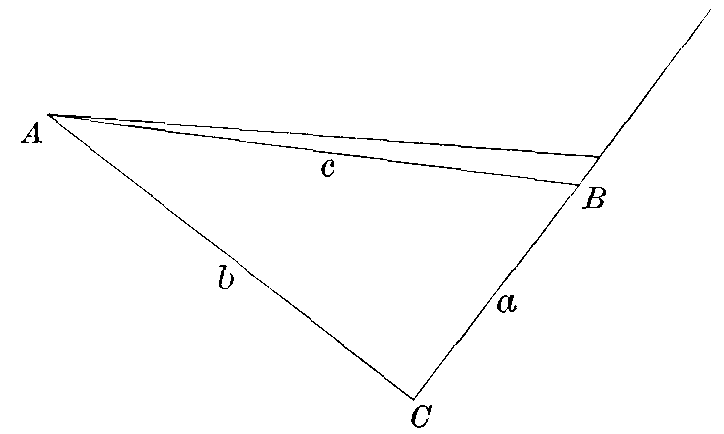
\includegraphics[width=60mm]{fig77.png}
\end{figure}

直角三角形 $ABC$ から、$b$ を固定したままにして、方程式
\begin{align*}
  \sin A &= \frac{\cos B}{\cos b}
\intertext{を微分すると、}
  dB &= -\cos c \,dA\tag{II.}
\end{align*}
を得る。

\begin{figure}[h]
\centering
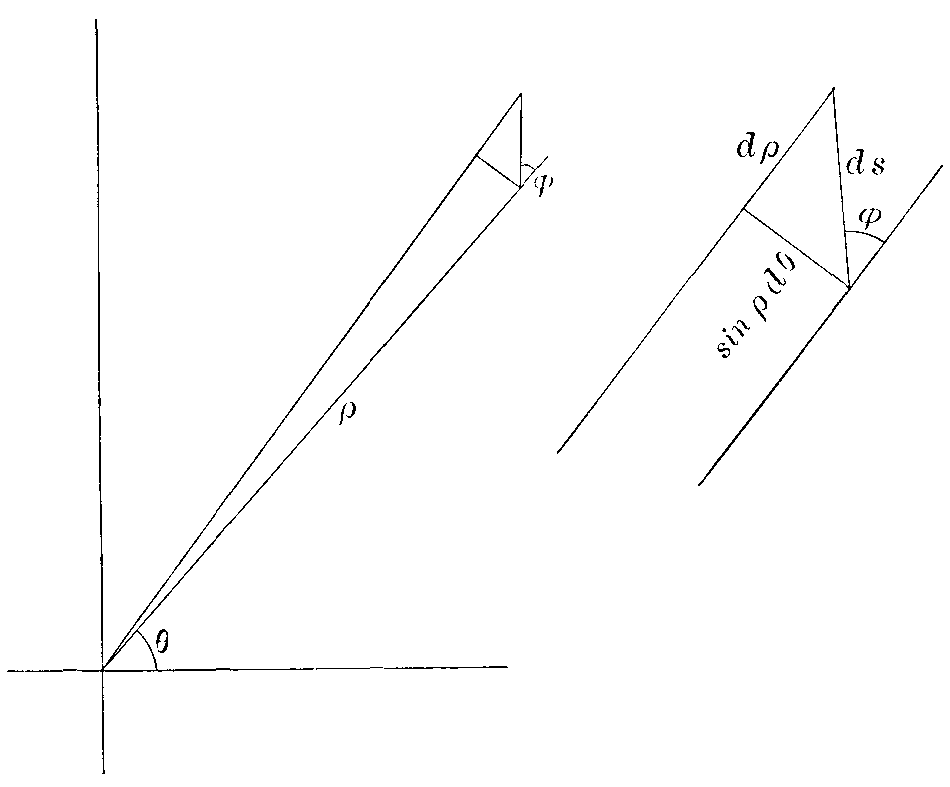
\includegraphics[width=80mm]{fig78.png}
\end{figure}

こうして、極座標での微分公式は、
\begin{align*}
  ds^2 &= d\rho^2 + \sin^2\rho\,d\theta^2,\\
  \tan\phi &= \sin\rho\, \frac{d\theta}{d\rho};\footnotemark
\intertext{直角に交わる二つの弧については}
  \frac{d\rho}{d\theta}\, \frac{d'\rho}{d'\theta} &= -\sin^2\rho
\end{align*}
である。
\footnotetext{ユークリッド幾何学の対数螺旋のように $\phi$ が定数であれば、この方程式を積分することができる。すなわち、
  \begin{align*}
    \tan\phi\, \frac{d\rho}{\sin\rho} &= d\theta.\\
    \therefore \tan\phi\, \log\tan\frac{\rho}{2} &= \theta+c,\\
    \intertext{すなわち}
    \tan\frac{\rho}{2} &= e^\frac{\theta+c}{\tan\phi}.\\
    \intertext{$e^\frac{c}{\tan\phi}$ を $c'$ と書くと、これは}
    \tan\frac{\rho}{2} &= c' e^\frac{\theta}{\tan\phi}
  \end{align*}
  となる。球面上では、これは斜航線と呼ばれる曲線である。}

面積の公式は、\footnote{面積の単位を適切に選ぶ。}
\begin{equation*}
  \iint \sin\rho\, d\rho\, d\theta
\end{equation*}
である。まず $\rho$ について積分する。面積が原点を含み、各動径が曲線とただ一度だけ交わるならば、この式は
\begin{equation*}
  2\pi - \int_0^{2\pi} \cos\rho\, d\theta
\end{equation*}
となる。

曲線を一周するときの全回転は、双曲の場合と同様にして求められ、
\begin{equation*}
  \int_0^{2\pi} \cos\rho\, d\theta
\end{equation*}
である。したがって、面積は、この回転が四直角に足りない量に等しい。

たとえば、半径 $\rho$ の円の面積は $2\pi(1-\cos\rho)$ であり、その一周で回転する量は $2\pi\cos\rho$ である。平面全体の面積は $2\pi$ である。

\item[7.~座標系の修正:]\hfill\break

$\tan x$ の代わりに $u$、$\tan y$ の代わりに $v$、$\tan\rho$ の代わりに $r$、などと書くと、
\begin{align*}
  u^2 + v^2 &= r^2.\footnotemark \\
\intertext{直線の方程式は}
  au + bv + 1 &= 0, \\
\intertext{となり、円の方程式は}
  (1 + u^2 + v^2)c^2 &= (1 + au + bv)^2
\end{align*}
となる。
\footnotetext{双曲の場合の脚注はここにも当てはまる。}
\end{description}

